%%
%% Beginning of file 'sample62.tex'
%%
%% Modified 2018 January
%%
%% This is a sample manuscript marked up using the
%% AASTeX v6.2 LaTeX 2e macros.
%%
%% AASTeX is now based on Alexey Vikhlinin's emulateapj.cls 
%% (Copyright 2000-2015).  See the classfile for details.

%% AASTeX requires revtex4-1.cls (http://publish.aps.org/revtex4/) and
%% other external packages (latexsym, graphicx, amssymb, longtable, and epsf).
%% All of these external packages should already be present in the modern TeX 
%% distributions.  If not they can also be obtained at www.ctan.org.

%% The first piece of markup in an AASTeX v6.x document is the \documentclass
%% command. LaTeX will ignore any data that comes before this command. The 
%% documentclass can take an optional argument to modify the output style.
%% The command below calls the preprint style  which will produce a tightly 
%% typeset, one-column, single-spaced document.  It is the default and thus
%% does not need to be explicitly stated.
%%
%%
%% using aastex version 6.2
\documentclass{aastex62}

%% The default is a single spaced, 10 point font, single spaced article.
%% There are 5 other style options available via an optional argument. They
%% can be envoked like this:
%%
%% \documentclass[argument]{aastex62}
%% 
%% where the layout options are:
%%
%%  twocolumn   : two text columns, 10 point font, single spaced article.
%%                This is the most compact and represent the final published
%%                derived PDF copy of the accepted manuscript from the publisher
%%  manuscript  : one text column, 12 point font, double spaced article.
%%  preprint    : one text column, 12 point font, single spaced article.  
%%  preprint2   : two text columns, 12 point font, single spaced article.
%%  modern      : a stylish, single text column, 12 point font, article with
%% 		  wider left and right margins. This uses the Daniel
%% 		  Foreman-Mackey and David Hogg design.
%%  RNAAS       : Preferred style for Research Notes which are by design 
%%                lacking an abstract and brief. DO NOT use \begin{abstract}
%%                and \end{abstract} with this style.
%%
%% Note that you can submit to the AAS Journals in any of these 6 styles.
%%
%% There are other optional arguments one can envoke to allow other stylistic
%% actions. The available options are:
%%
%%  astrosymb    : Loads Astrosymb font and define \astrocommands. 
%%  tighten      : Makes baselineskip slightly smaller, only works with 
%%                 the twocolumn substyle.
%%  times        : uses times font instead of the default
%%  linenumbers  : turn on lineno package.
%%  trackchanges : required to see the revision mark up and print its output
%%  longauthor   : Do not use the more compressed footnote style (default) for 
%%                 the author/collaboration/affiliations. Instead print all
%%                 affiliation information after each name. Creates a much
%%                 long author list but may be desirable for short author papers
%%
%% these can be used in any combination, e.g.
%%
%% \documentclass[twocolumn,linenumbers,trackchanges]{aastex62}
%%
%% AASTeX v6.* now includes \hyperref support. While we have built in specific
%% defaults into the classfile you can manually override them with the
%% \hypersetup command. For example,
%%
%%\hypersetup{linkcolor=red,citecolor=green,filecolor=cyan,urlcolor=magenta}
%%
%% will change the color of the internal links to red, the links to the
%% bibliography to green, the file links to cyan, and the external links to
%% magenta. Additional information on \hyperref options can be found here:
%% https://www.tug.org/applications/hyperref/manual.html#x1-40003
%%
%% If you want to create your own macros, you can do so
%% using \newcommand. Your macros should appear before
%% the \begin{document} command.
%%

\usepackage{graphicx}
\usepackage{float}
\usepackage[caption=false]{subfig}
\usepackage{enumitem}

%\usepackage{natbib}
%\usepackage{pdflscape}

%% AASTeX v6.* now includes \hyperref support. While we have built in specific
%% defaults into the classfile you can manually override them with the
%% \hypersetup command. For example,
%%
%%\hypersetup{linkcolor=red,citecolor=green,filecolor=cyan,urlcolor=magenta}
%%
%% will change the color of the internal links to red, the links to the
%% bibliography to green, the file links to cyan, and the external links to
%% magenta. Additional information on \hyperref options can be found here:
%% https://www.tug.org/applications/hyperref/manual.html#x1-40003

%% If you want to create your own macros, you can do so
%% using \newcommand. Your macros should appear before
%% the \begin{document} command.
%%
\newcommand{\vdag}{(v)^\dagger}
\newcommand\aastex{AAS\TeX}
\newcommand\latex{La\TeX}
\newcommand{\exampleConstant}{0.04}
\newcommand{\degree}{^\circ}
\newcommand{\spitzer}{{\it Spitzer}}
\newcommand{\kepler}{{\it Kepler}}

%% Reintroduced the \received and \accepted commands from AASTeX v5.2
%\received{July 1, 2016}
%\revised{September 27, 2016}
%\accepted{\today}
%% Command to document which AAS Journal the manuscript was submitted to.
%% Adds "Submitted to " the arguement.
%\submitjournal{ApJ}

%% Mark up commands to limit the number of authors on the front page.
%% Note that in AASTeX v6.1 a \collaboration call (see below) counts as
%% an author in this case.
%
%\AuthorCollaborationLimit=3
%
%% Will only show Schwarz, Muench and "the AAS Journals Data Scientist 
%% collaboration" on the front page of this example manuscript.
%%
%% Note that all of the author will be shown in the published article.
%% This feature is meant to be used prior to acceptance to make the
%% front end of a long author article more manageable. Please do not use
%% this functionality for manuscripts with less than 20 authors. Conversely,
%% please do use this when the number of authors exceeds 40.
%%
%% Use \allauthors at the manuscript end to show the full author list.
%% This command should only be used with \AuthorCollaborationLimit is used.

%% The following command can be used to set the latex table counters.  It
%% is needed in this document because it uses a mix of latex tabular and
%% AASTeX deluxetables.  In general it should not be needed.
%\setcounter{table}{1}

%%%%%%%%%%%%%%%%%%%%%%%%%%%%%%%%%%%%%%%%%%%%%%%%%%%%%%%%%%%%%%%%%%%%%%%%%%%%%%%%
%%
%% The following section outlines numerous optional output that
%% can be displayed in the front matter or as running meta-data.
%%
%% If you wish, you may supply running head information, although
%% this information may be modified by the editorial offices.
\shorttitle{NIRCam Lab Stability Studies}
\shortauthors{Schlawin et al.}
%%
%% You can add a light gray and diagonal water-mark to the first page 
%% with this command:
% \watermark{text}
%% where "text", e.g. DRAFT, is the text to appear.  If the text is 
%% long you can control the water-mark size with:
%  \setwatermarkfontsize{dimension}
%% where dimension is any recognized LaTeX dimension, e.g. pt, in, etc.
%%
%%%%%%%%%%%%%%%%%%%%%%%%%%%%%%%%%%%%%%%%%%%%%%%%%%%%%%%%%%%%%%%%%%%%%%%%%%%%%%%%

%% This is the end of the preamble.  Indicate the beginning of the
%% manuscript itself with \begin{document}.

\begin{document}

\title{Lessons Learned for JWST Transiting Planet Time Series from Ground-based Studies of the NIRCam Detectors}

%% LaTeX will automatically break titles if they run longer than
%% one line. However, you may use \\ to force a line break if
%% you desire. In v6.1 you can include a footnote in the title.

%% A significant change from earlier AASTEX versions is in the structure for 
%% calling author and affilations. The change was necessary to implement 
%% autoindexing of affilations which prior was a manual process that could 
%% easily be tedious in large author manuscripts.
%%
%% The \author command is the same as before except it now takes an optional
%% arguement which is the 16 digit ORCID. The syntax is:
%% \author[xxxx-xxxx-xxxx-xxxx]{Author Name}
%%
%% This will hyperlink the author name to the author's ORCID page. Note that
%% during compilation, LaTeX will do some limited checking of the format of
%% the ID to make sure it is valid.
%%
%% Use \affiliation for affiliation information. The old \affil is now aliased
%% to \affiliation. AASTeX v6.1 will automatically index these in the header.
%% When a duplicate is found its index will be the same as its previous entry.
%%
%% Note that \altaffilmark and \altaffiltext have been removed and thus 
%% can not be used to document secondary affiliations. If they are used latex
%% will issue a specific error message and quit. Please use multiple 
%% \affiliation calls for to document more than one affiliation.
%%
%% The new \altaffiliation can be used to indicate some secondary information
%% such as fellowships. This command produces a non-numeric footnote that is
%% set away from the numeric \affiliation footnotes.  NOTE that if an
%% \altaffiliation command is used it must come BEFORE the \affiliation call,
%% right after the \author command, in order to place the footnotes in
%% the proper location.
%%
%% Use \email to set provide email addresses. Each \email will appear on its
%% own line so you can put multiple email address in one \email call. A new
%% \correspondingauthor command is available in V6.1 to identify the
%% corresponding author of the manuscript. It is the author's responsibility
%% to make sure this name is also in the author list.
%%
%% While authors can be grouped inside the same \author and \affiliation
%% commands it is better to have a single author for each. This allows for
%% one to exploit all the new benefits and should make book-keeping easier.
%%
%% If done correctly the peer review system will be able to
%% automatically put the author and affiliation information from the manuscript
%% and save the corresponding author the trouble of entering it by hand.

\correspondingauthor{Everett Schlawin}
\email{eas342 AT EMAIL Dot Arizona .edu}

\author[0000-0001-8291-6490]{Everett Schlawin}
\affiliation{Steward Observatory \\
933 North Cherry Avenue \\
Tucson, AZ 85721, USA}

\author{Rafia Bushra}
\affiliation{Steward Observatory \\
933 North Cherry Avenue \\
Tucson, AZ 85721, USA}

\author{Stephanie Striegel}
\affiliation{Department of Physics \& Astronomy \\
San Jose State University \\
One Washington Square \\
San Jose, CA 95192, USA}
\affiliation{NASA Ames Research Center \\
Space Science and Astrobiology Division \\
Moffett Field, CA 94035, USA}

\author{Xander Levinson}
\affiliation{Department of Astronomy \& Astrophysics \\
University of California, Santa Cruz \\
1156 Highland Street \\
Santa Cruz, CA 95062, USA}
\affiliation{NASA Ames Research Center \\
Space Science and Astrobiology Division \\
Moffett Field, CA 94035, USA}

\author{Jarron Leisenring}
\affiliation{Steward Observatory \\
933 North Cherry Avenue \\
Tucson, AZ 85721, USA}

\author{Karl Misselt}
\affiliation{Steward Observatory \\
933 North Cherry Avenue \\
Tucson, AZ 85721, USA}

\author{Douglas Kelly}
\affiliation{Steward Observatory \\
933 North Cherry Avenue \\
Tucson, AZ 85721, USA}

\author{Thomas Beatty}
\affiliation{Steward Observatory \\
933 North Cherry Avenue \\
Tucson, AZ 85721, USA}



\author{Thomas P Greene}
\affiliation{NASA Ames Research Center \\
Space Science and Astrobiology Division \\
Moffett Field, CA 94035, USA}

\author{Marcia Rieke}
\affiliation{Steward Observatory \\
933 North Cherry Avenue \\
Tucson, AZ 85721, USA}


%% Note that the \and command from previous versions of AASTeX is now
%% depreciated in this version as it is no longer necessary. AASTeX 
%% automatically takes care of all commas and "and"s between authors names.

%% AASTeX 6.1 has the new \collaboration and \nocollaboration commands to
%% provide the collaboration status of a group of authors. These commands 
%% can be used either before or after the list of corresponding authors. The
%% argument for \collaboration is the collaboration identifier. Authors are
%% encouraged to surround collaboration identifiers with ()s. The 
%% \nocollaboration command takes no argument and exists to indicate that
%% the nearby authors are not part of surrounding collaborations.

%% Mark off the abstract in the ``abstract'' environment. 
\begin{abstract}

JWST transmission and emission spectra of transiting exoplanets will provide invaluable glimpses at exoplanet atmospheres.
These spectra will reveal the composition and temperature structure at a level never achieved before.
This promising science from JWST, however, will require exquisite precision and understanding of systematic errors that can impact the time series of planets crossing in front of and behind their host stars.
This is especially true if JWST is used to search for biosignatures in temperature atmospheres on Earth-sized planets that may contain liquid water.
Here, we provide the lessons learned from ground-based characterization of the NIRCam H2RG detector, which will be used for exoplanet spectra.
%and are the same type of detectors used in JWST's NIRISS and NIRSpec instruments.
We summarize the lessons learned from tests at NASA Goddard, NASA Johnson and the University of Arizona detector labs.

\end{abstract}

%% Keywords should appear after the \end{abstract} command. 
%% See the online documentation for the full list of available subject
%% keywords and the rules for their use.
\keywords{stars: atmospheres --- stars: individual (\objectname{KIC 12557548}) ---
stars: variables: general}

%% From the front matter, we move on to the body of the paper.
%% Sections are demarcated by \section and \subsection, respectively.
%% Observe the use of the LaTeX \label
%% command after the \subsection to give a symbolic KEY to the
%% subsection for cross-referencing in a \ref command.
%% You can use LaTeX's \ref and \label commands to keep track of
%% cross-references to sections, equations, tables, and figures.
%% That way, if you change the order of any elements, LaTeX will
%% automatically renumber them.

%% We recommend that authors also use the natbib \citep
%% and \citet commands to identify citations.  The citations are
%% tied to the reference list via symbolic KEYs. The KEY corresponds
%% to the KEY in the \bibitem in the reference list below. 

\section{Introduction} \label{sec:intro}

JWST will provide powerful new measurements of exoplanet atmospheres with spectroscopy from 0.6 to 12 $\mu$m
\citep{beichman2014pasp,greene2016jwst_trans,howe2017informationJWST,barstow2015jwstSystematics,schlawin2018JWSTforecasts}.
The sensitivity of JWST combined with its unprecedented wavelength coverage on exoplanets will enable it to measure the abundance of carbon-bearing molecules (CO, CO$2$ and CH$_4$) as well as study cooler, smaller planets than previously characterized.

JWST has also been considered for observations of potentially habitable Earth-like planets that orbit their stars at a distance where water could be in liquid form on their surface.
The TRAPPIST-1 system \citep{gillon2016trappist1Discovery,gillon2017trappist-1sevenp} presents an exciting opportunity to study Earth-sized stars orbiting a 0.1~R$_\odot$ M-type star.
By putting together 10 to 30 transits, it will be possible to collect enough photons to detect CO$_2$ \citep{barstow2016trappist1habitable,krissansen-totton2018trappist1eJWST}.
Optimistically, 30 transits may contain enough photons to detect O$_3$ in the atmosphere of TRAPPIST-1 d with JWST if clouds have a minimal impact on its atmosphere \citep{barstow2016trappist1habitable}.
Alternatively, 10 transits of TRAPPIST-1e could be sufficient study if the planet's atmosphere has CO$_2$ and CH$_4$ biosignatures similar to early-Earth \citep{krissansen-totton2018trappist1eJWST}.
A critical question in studying planets like TRAPPIST-1 d/e, however, is whether photon-limited performance is possible with JWST observations.

Experience with the Hubble Space Telescope (HST), \spitzer, and \kepler\ shows that many systematics can affect high precision time series and prevent photon-limited performance unless corrected for \citep[e.g.][]{beichman2014pasp}.
Many of these effects are detector-related including charge trapping on HST's detector \citep{berta2012flat_gj1214,zhou2017chargeTrap}, intra-pixel sensitivity on the short wavelength bands of \spitzer\ IRAC \citep{moralesCalderon2006LdwarfsWeatherIPC} and sensitivity to pointing jitter with \kepler\footnote{https://keplerscience.arc.nasa.gov/K2/Performance.shtml} \citep{beichman2014pasp}.

The NIRCam instrument \citep{rieke2005nircamSPIE} contains a slitless grism mode with its long wavelength channel \citep{greene2017jatisNIRCam}.
This slitless grism mode is analogous to the WFC3 grism on HST that has been successfully employed on many transiting planets \citep[e.g.][]{deming13,kreidberg2014wasp43,sing2016continuum,wakeford2017hatp26}.
The NIRCam grism mode will collect moderate resolution R$\sim$1100-1700 spectra over the wavelength range from 2.4 to 5.0~$\mu$m.
This grism mode can be used simultaneously with short wavelength weak lens imaging or the Dispersed Hartmann Sensor mode \citep{schlawin2017dhs}. If it becomes an approved and implemented mode, the DHS will permit spectroscopy simultaneous from 1.0 to 2.0~$\mu$m because of a dichroic beamsplitter that divides the light from NIRCam into two different channels.
The DHS mode will permit time series spectroscopy on very bright targets ($K_S \sim 1$) inaccessible by other modes.

Section \ref{sec:detectorPrimer} gives a review of NIRCam's detector operation.
Section \ref{sec:knownEffects} lists the known systematic effects that can impeded high precision time series and increase the noise above the photon and read noise.
Section \ref{sec:experiments} describes the experiments on the ground that are used to prepare for JWST observations in flight.


\section{A Primer on Detector Operation}\label{sec:detectorPrimer}

\subsection{Photosensitive Operation}
\textcolor{red}{\textbf{NOTE: This section needs checking for factual accuracy by a detector expert}}

It is helpful to review the basic operation of a NIRCam detector in order to understand the systematics affecting time series \citep[e.g.][]{rieke2007irDetectorReview}.
Figure \ref{fig:npSchematic} shows a schematic of an NP semiconductor junction for a H2RG detector from \citet{smith2008imgPersistence}.
The crystalline HgCdTe structure has 4 valence electrons that form covalent bonds in a tetrahedral structure.
By varying the relative amount of Hg, Cd and Te (doping), it is possible to increase or decrease the number of electrons to create mobile charge carriers that move along the crystaline lattice.
The N-type semiconductor is a negatively-doped HgCdTe crystalline structure that has negative charge carriers (electrons).
The P-type semiconductor is a positively-doped HgCdTe crystalline structure that has positive charge carriers (vacant holes in the lattice structure than can move like electrons).

\begin{figure}[!hbtp]
\centering
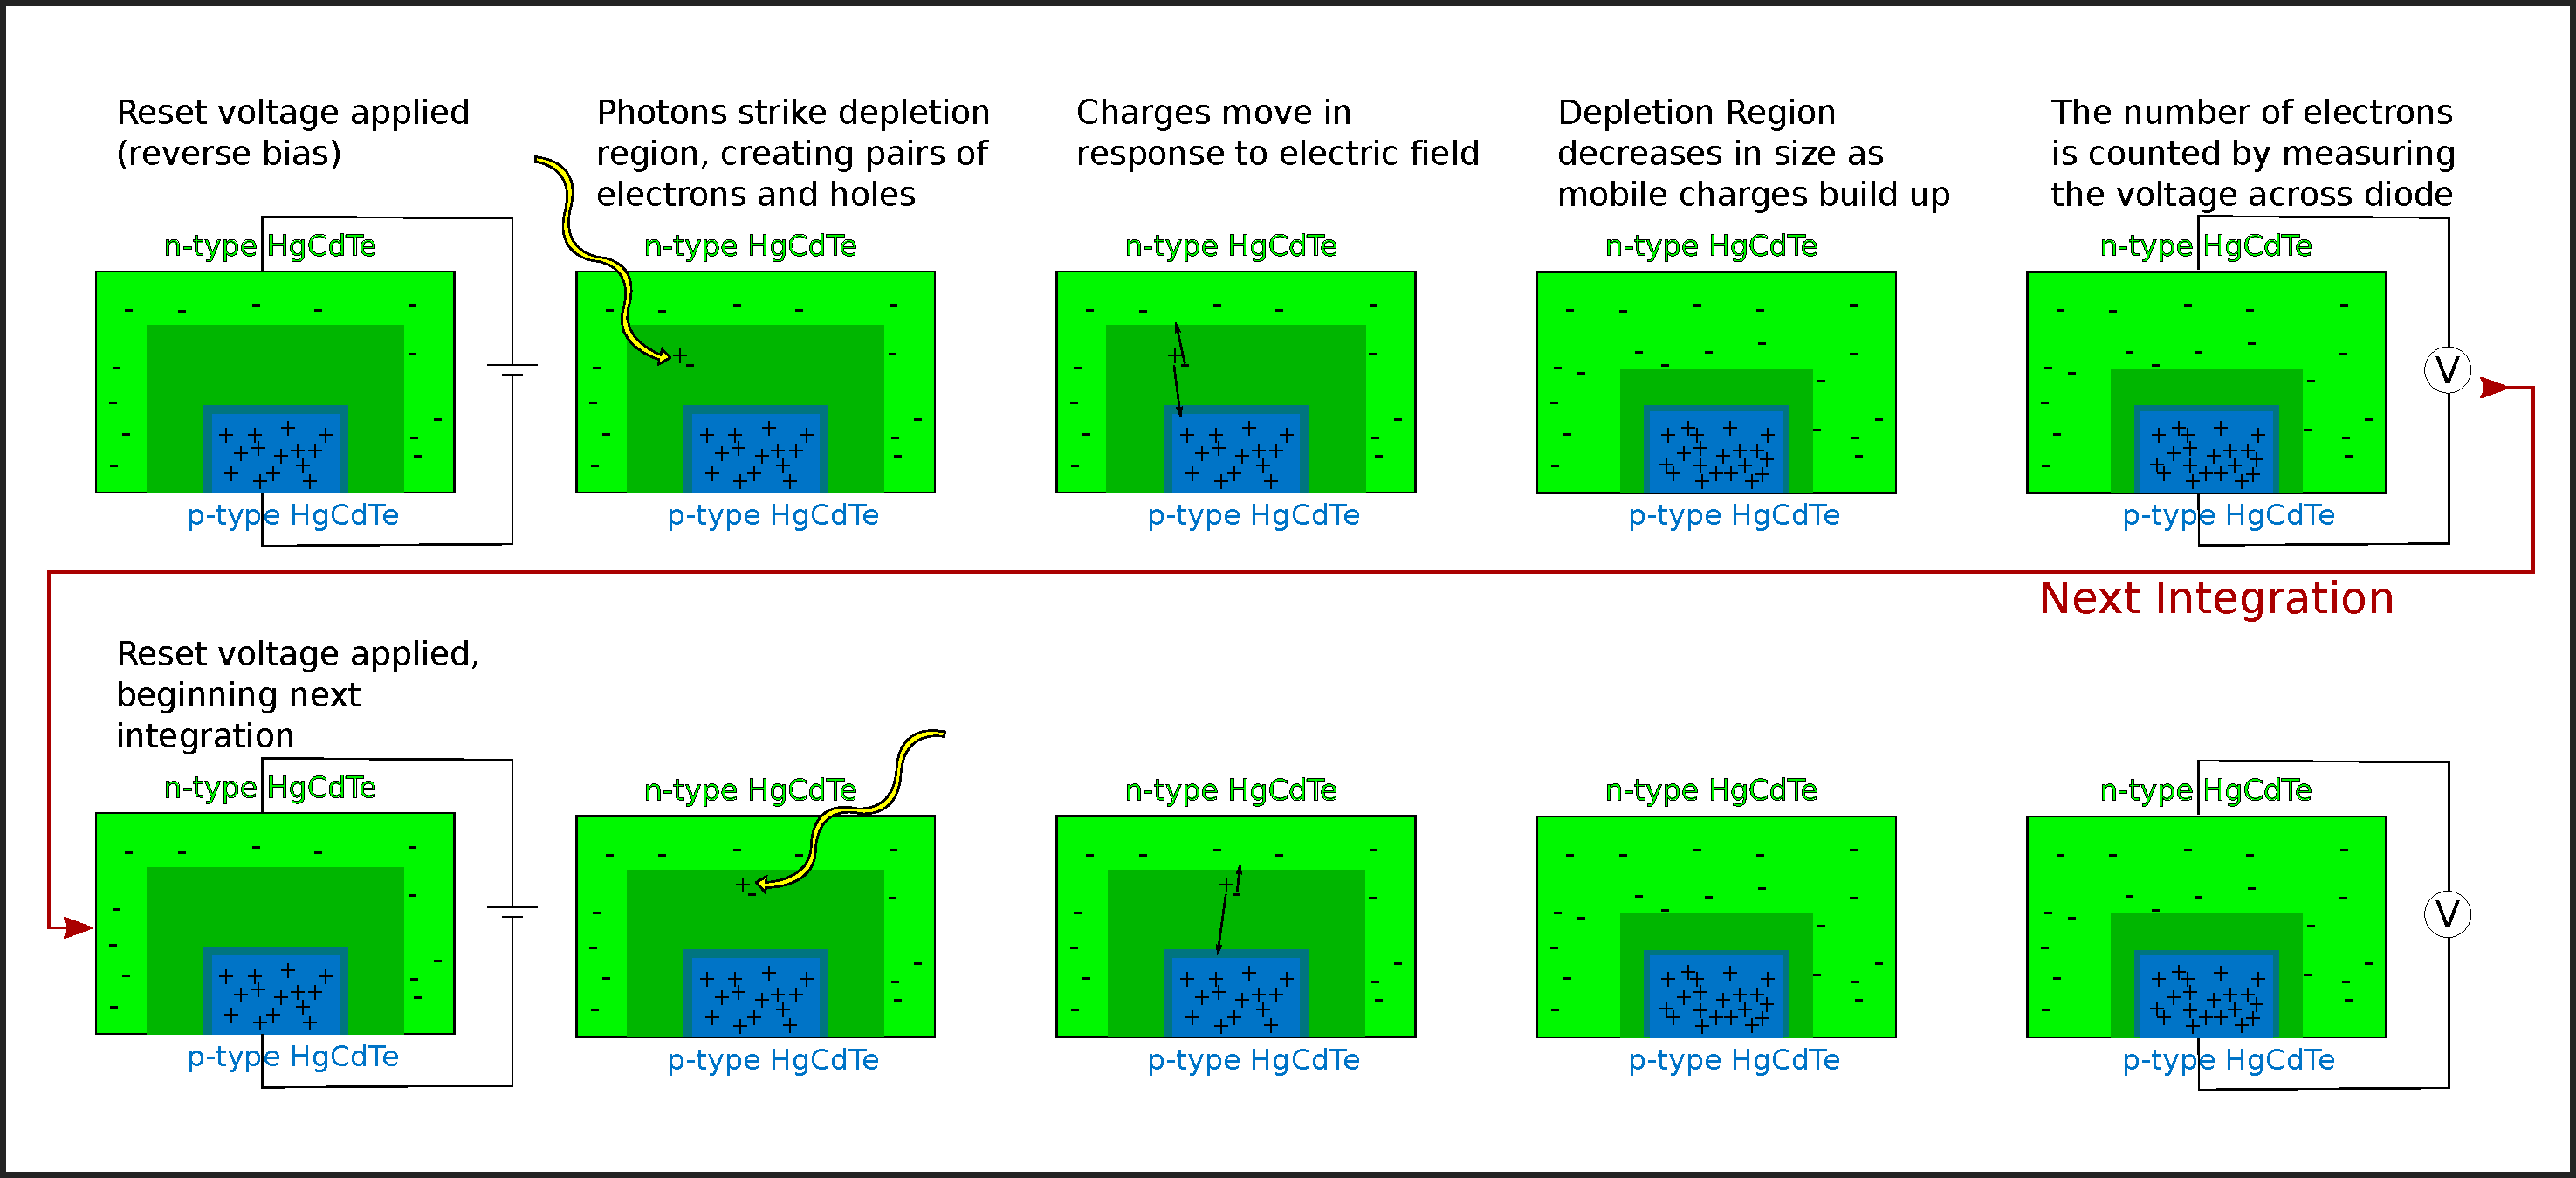
\includegraphics[width=.99\columnwidth]{ideal_photodiode.pdf}
\caption{A cartoon schematic of a H2RG detector inspired by \citet{smith2008imgPersistence} and \citet{tulloch2018persistenceH2RG}.
The green and blue regions depict the N-type and P-type semiconductors.
The undepleted zones of the semiconductor (fire brick and dim gray colors) contain mobile charge carriers whereas the depletion region (dark salmon) has no mobile carriers and all electrons are in the valence state.
The depletion region is widest after detector reset and shrinks as the detector is illuminated with photons that create electron-hole pairs.
The voltage can be measured non-destructively as the well fills and then reset before saturating.}\label{fig:npSchematic}
\end{figure}



The junction of these two materials enables electrons to flow from the N-type material to the P-type material where it can complete a valence shell in the semiconductor material.
This produces a negative charge on the P-type side.
Conversely, the positively charged holes from the P-type material flow to the N-type material to complete the valence shell and this produces a positive charge.
This difference is called the contact potential.
In the region where electrons have completed the valence shells in the P-type material and holes in the N-type material, the valence shells are complete.
This region spanning across the two semiconductor materials is called the depletion region, because it contains no mobile charge carriers.
The positive net charge on the N-type material and negative charge in the P-type material causes a voltage (potential) difference across the detector.

The NP junction in Figure \ref{fig:npSchematic} is ``reverse-biased'' with a positive potential on the N-type material and negative potential on the P-type.
The positive potential on the N-type material attracts the negative charge carriers (electrons) whereas the negative potential on the P-type material attracts the  positve charge carriers (holes).
The reverse bias thus reduces the number of mobile charge carriers and increases the size of the depletion region.
The increased depletion region size also increases the well depth or capacity of electrons that the detector may collect before saturation.
The reverse bias is applied at each reset at the beginning of a detector's integration.
Figure \ref{fig:npSchematic} shows the case where the density of charge carriers is equal in the N-type and P-type semiconductors, but in reality, the density of the P-type semiconductor is much higher than the N-type, so the depletion region has a larger physical size on the N-type side.

Note that Figure \ref{fig:npSchematic} shows the mobile charge carriers only, so the depletion region, with no mobile charges is positively charged on the N-type side and negatively charged on the P-type side.
The undepleted region is electrically neutral because the nuclei of the N-type material have an equal number of extra protons as the negatively charged electrons.
Similarly, the undepleted region of the P-type semiconductor has fewer protons in its atomic nuclei producing an overall neutral charge.
Textbook NP junction schematics often show the net charge and thus symbolize the regions with charge carriers as empty and the depletion region with ``+'' symbols on the N-type semiconductor and ``-'' symbols on the P-type˚ \citep[e.g.][]{halliday2004physicsText}.
The schematic in Figure \ref{fig:npSchematic} instead shows the mobile charge carriers as ``+'' and ``-'' because it is easier to visualize the charge trapping effect this way \citep[e.g.][]{smith2008imgPersistence}.

When an incoming photon strikes the N-type depletion region, it will excite an electron from the valence to conduction band which creates an electron-hole pair \citep{rieke2007irDetectorReview}.
The electron moves to the extremity of the depletion zone in the N-type material whereas the positive hole generated crosses the NP junction and adds a mobile charge to the P-type side.
The incoming photon has the effect of decreasing the size of the depletion region.
A second photon will excite another electron-hole pair so that a hole moves to the P-type side.
This continues and decreases the size of the depletion region.
The diffusion of charge carriers across the junction changes the voltage across the NP junction, which can be measured with a sensitive amplifier circuit.

As the size of the depletion region decreases, the detector becomes decreasingly sensitive to new photons.
Thus, the NIRCam HgCdTe detectors are never strictly linear.
Eventually, with enough photons, the depletion region is too small to create electron-hole pairs with incoming photons.
This is where the detector approaches saturation and no longer changes voltage with more light.

\subsection{Readout Circuit}\label{sec:readout}

The accumulated charge from absorbed photons in the detector is measured with a multiplexor (MUX) that form a readout integrated circuit (ROIC) \citep{rieke2007irDetectorReview}.
This readout circuitry makes allows the signal to be measured non-destructively up the ramp in so-called ``multiaccum" mode.

A sensitive amplifier converts the measured voltage potential (as compared with the bias level after reset) into a signal.
The electronic circuit that digitizes the voltages is tuned to ensure the 16 bits (65,536 possible Data Numbers) measure the voltage across the NP junction from the value just after reset (before photons are detected) to the saturation voltage where the maximum number of photons are collected and no more electron-hole pairs can be produced in the depletion region.
The minimum voltage is several thousands of counts above zero to ensure that fluctuations in the bias signal do not below 0.
The 65,536 DN level is tuned to be just above the HgCdTe full well capacity to measure full saturation.




\section{Known Detector Effects}\label{sec:knownEffects}

Known detector effects that could affect stability include:
\begin{itemize}[noitemsep]
	\item \textbf{Intrapixel sensitivity:} - including sub-pixel flat fielding issues and sub-pixel crosshatching on the detectors \citep{shapiro2018crosshatch}
	\item \textbf{Pre-amp reset offsets:} (an Asic-related effect) 
The resets cause discontinuities in the pedestal level of all pixels between frames. This is an effect where averaging over more pixels does not decrease the noise, but reference pixel or background subtraction can. These are discussed in Section \ref{sec:preAmp}.
	\item \textbf{1/f noise:} This is a noise source where most of the noise power is concentrated as low frequencies. 1/f noise causes spatial correlations in the fast-read direction (along detector rows). It is highly correlated between amplifiers, suggesting that it is caused by a common reference voltage. 1/f noise is efficiently removed by reference pixels
	\item \textbf{Even/odd offsets:} Alternating columns have different bias levels. Additionally, there are offsets between columns that can change from frame to frame, especially on NIRCam's LW detector
	\item \textbf{kTC noise:} A random process due to the unknown amount of charge stored at the reset voltage level
	\item \textbf{Detector Temperature Fluctuations:} The JWST detectors are sensitive to temperature changes on the detectors. For example, laboratory tests show that 100 mK temperature fluctuations can result in $\sim$ 80 ADU changes on the detector that are not corrected by reference pixels \citep{hall2005jwstArrays}. Fortunately, the detectors are actively thermally controlled to keep the temperature fluctuations to $\lesssim$ 1 mK.
	\item \textbf{ASIC Temperature Fluctuations:} The asic temperature will change as the operating mode. For example, in the CV3 stability test, the temperature of the A asic changed by $\sim$80 mK when the readout mode was switched from full frame to subarray. This temperature change is expected to be smaller in flight due to adjustments in ?? (Marcia said in 2018-11-02 meeting)
	\item \textbf{Elevated Columns} There is correlated noise along a column in many frames. These elevated columns can sometimes even move with time.
	\item \textbf{Random Telegraph Noise (RTN)} Some of the pixels will exhibit spontaneous changes jumps in signal even with no illumination. Fortunately, RTN appears in only $\sim$1000 pixels out of 4$\times 10^6$ on the array.
	\item \textbf{Detector Fringing} \textbf{\textcolor{red}{Add more details and citations}} The thin $\sim 5\mu$m layers of the H2RG detectors will cause interference patterns on the array due to constructive and destructive interference of light at wavelengths similar to the thickness of the layers. If the detector fringe pattern changes with time, it will change the throughput of a grism image.
	\item \textbf{Amplifier Boundary Discontinuities} The NIRCam detectors can be read out in full frame, stripe and window modes. The full frame and stripe modes make use of 4 amplifiers that can record or reset the accumulated electrons in 4 pixels simultaneously in parallel. The parallel operation of the amplifiers reduces the frame time and reset time by a factor of 4 but can introduce subtle voltage biases between regions of the detector. If these voltage biases are not corrected, they can potentially introduce discontinuities in a spectrum, which crosses amplifier boundaries.
\end{itemize}

It should be noted that the detector effects related to the asic circuit can be specific to the ``personality'' of each asic. The asics all have different asic load files which are tuned to minimize the power consumption and dark current in a particular asic. Since the asic load files are specific to each detector, they may exhibit different noise properties.
Some caution should be taken when comparing noise tests with engineering grade or rejected detectors with the flight detectors.

\subsection{Pre-amp Reset Offsets from the Lockheed CV Test}\label{sec:preAmp}

The NIRCam detectors' pre-amplifiers (pre-amps) have a reference voltage that can drift with time.
This can affect the pedestal level of all pixels over long ($\gtrsim$ 20 minute timescales).
These pre-amplifier levels can either be reset at the beginning of an integration with samples up the ramp or with each frame up the ramp.
The NIRCam detectors are usually set to reset once per frame to prevent large amplifier drifts over an integration \citep{robberto2014refPixPreAmp}.
However, one set of darks was collected at Lockheed CV with a reset only once per integration to study the effects of the pre-amplifier resets.

In the Lockheed CV test, the pedestal level of all pixels could be seen to drift over 19.3 minute dark integrations by 5 to 100 DN.
The drift was usually linear over these 19 minute exposures, but in one case was observed to drift downward from 100 DN to -50 DN and back to 100 DN \citep{robberto2014refPixPreAmp}.
The timescales for pre-amp resets are relevant to exoplanet time series, which have transit durations of $\sim$0.5 to 3 hours for typical targets.
However, reference pixel subtraction can efficiently remove pre-amp drifts, so with proper data reduction and subarrays that include reference pixels, the pre-amp drifts can be dramatically reduced.
It is also likely that background subtraction can mitigate the pre-amp reset offsets from time series integrations.
The NIRCam grism subarrays and dispersed source location are placed at the edge of the NIRCam Long Wavelength detector to ensure reference pixels are saved with active pixels.

\begin{figure}[!hbtp]
\centering
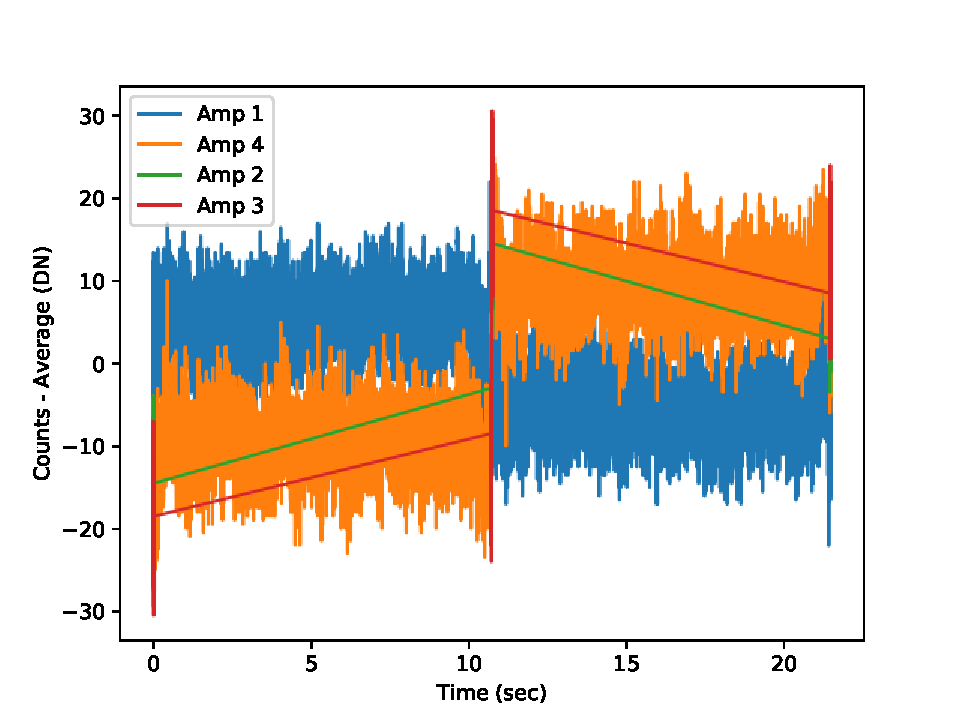
\includegraphics[width=.49\columnwidth]{allamps.pdf}
\includegraphics[width=.49\columnwidth]{allamps_long_dark.pdf}
\caption{Reference pixel time series for a two frame integration (Left) and a long dark integration of 108 frames (Right). Each of the plots show that the pre-amplifier resets between frames in an integration cause discontinuities in the reference signal. Amplifiers 1 and 4 track the time all through a frame with the side reference pixels, whereas amplifiers 2 and 3 in the middle only contain information on the bottom and top reference pixels at the beginning and ending of a frame.
The long dark exposure example of 108 integrations shows the behavior over long timescales.}\label{fig:ampResetDark}
\end{figure}

\subsection{Charge Trapping}
All HgCdTe detectors show a signal after bright illumination even if the illumination is removed; this is called persistence.
The physical mechanism that explain persistence is that charges are trapped in the depletion region after illumination by photons as the detector well fills \citep{smith2008imgPersistence,leisenring2016persistence}.
After the reverse-bias voltage is applied (a reset) in an ideal detector, the depletion region will be devoid of mobile charge carriers (electrons and holes).
However, in real detectors, some charges are trapped within the depletion region.
During a future integration, these charges will be released and shrink the size of the depletion region, filling a pixel with spurious signal (Data Numbers) not related to that integration's illumination by photons.
Figure \ref{fig:npSchematicTraps} shows how the size of the depletion region changes after charges have been released, highlighted with red circles.
The persistence from trapped charge is visible after an illumination by a source, where a residual image of a bright star can appear in dark regions or dark frames following the illumination.

the depletion region contains mobile charge carriers 
These charge traps will keep electrons and holes in the depletion region even after detector reset.
These traps then will release the charge at later times, which will create an artificial signal that affects the measured voltage the same way that incoming photons strike the depletion region.

The NIRCam detector shows low levels of persistence compared to previous generation detectors.

\begin{figure}[!hbtp]
\centering
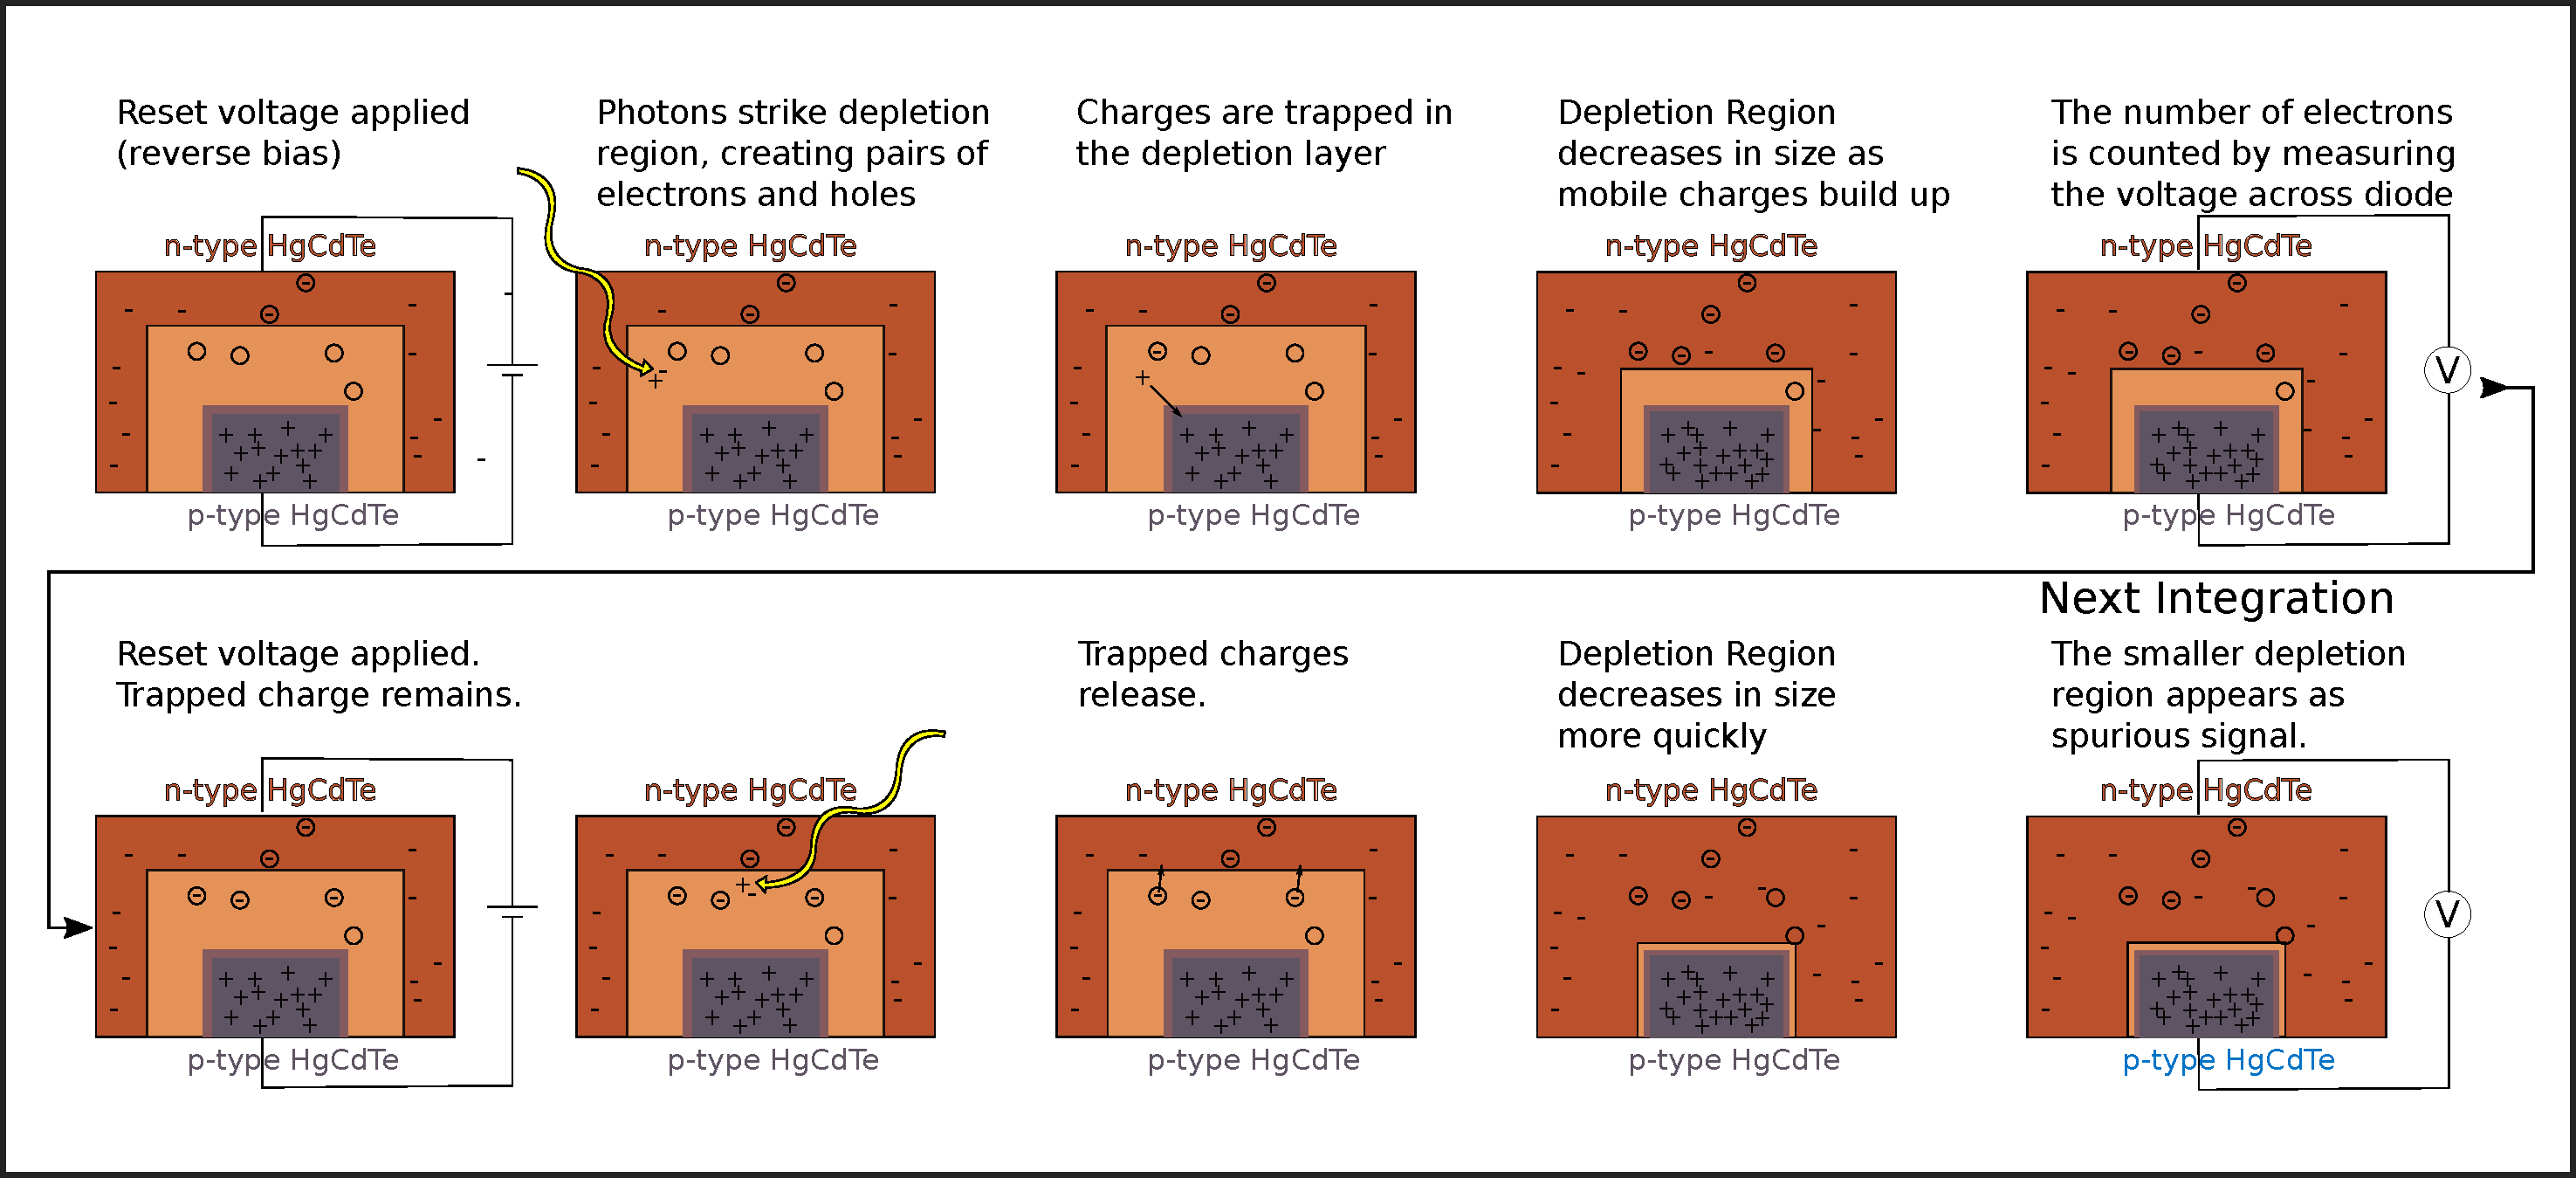
\includegraphics[width=.99\columnwidth]{charge_traps_photodiode.pdf}
\caption{A cartoon schematic of a H2RG detector with charge traps inspired by \citet{smith2008imgPersistence}, \citet{tulloch2018persistenceH2RG} and \citet{leisenring2016persistence}.
Charged traps for negative and positive carriers (depicted as round circles) will capture charge before it can flow to the undepleted regions of the detector.
The charge traps do not immediately empty with a detector reset, but instead release at later times causing a spurious signal.
This spurious signal (the shrinking of the depletion region as highlighted with red circles), causes a voltage change in future integrations that appears the same as a true signal from incoming photons.}\label{fig:npSchematicTraps}
\end{figure}

\subsection{Amplifier Boundary Discontinuities}
\begin{figure}[!hbtp]
\centering
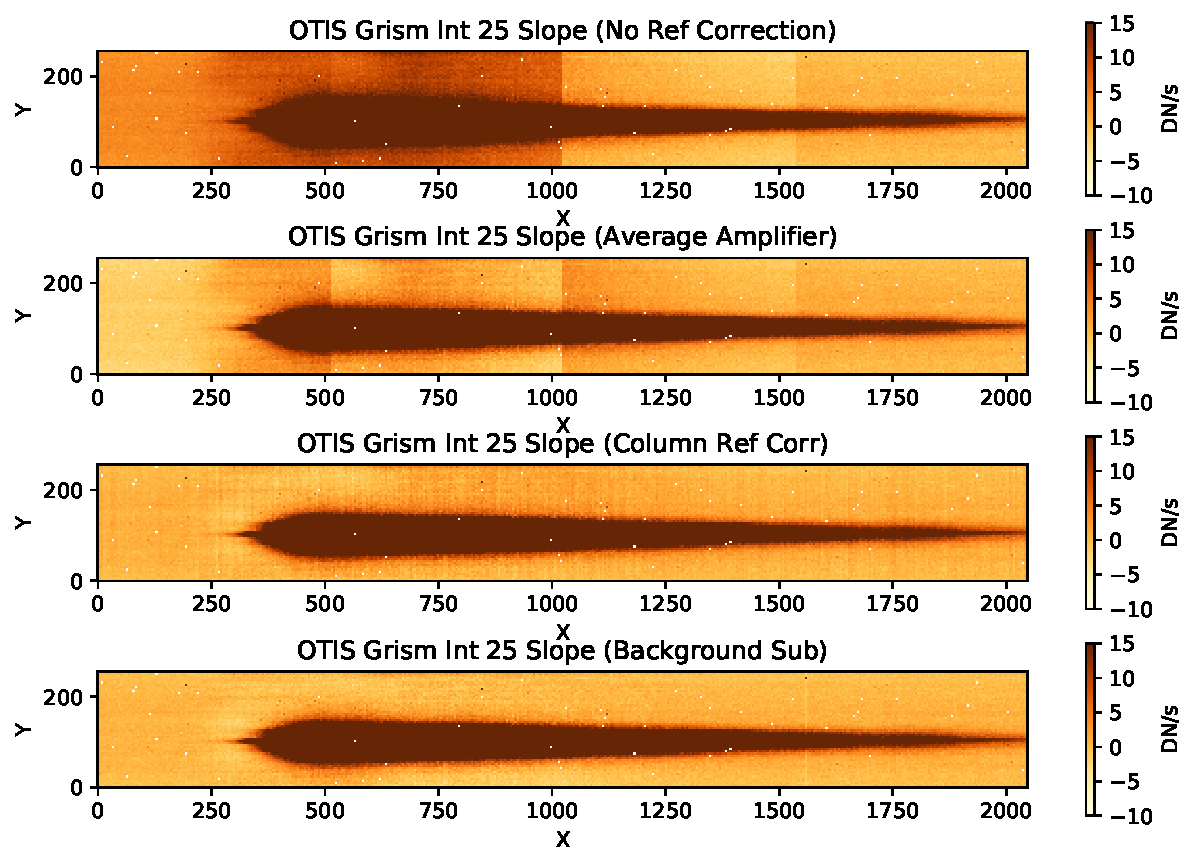
\includegraphics[width=.99\columnwidth]{amplifier_offsets_in_otis_lw_grism.pdf}
\caption{An example slope image from the LW OTIS Stability test.
{\it Top Panel:} No reference pixel correction is applied, leaving offsets at the amplifier boundaries.
{\it Middle Panel:} Reference pixel correction significantly reduces offsets between ampifiers.
{\it Bottom Panel:} The integrated flux (without background subtraction) shows substantially offsets in flux that are eliminated by reference pixel correction.
}\label{fig:ampOffsetsOtisGrismSlope}
\end{figure}



\section{Ground-based Experiments}\label{sec:experiments}

Table \ref{tab:testSummary} shows a summary of the ground-based tests that were performed on NIRCam detectors.
The flight NIRCam detectors, controllers, electronics, optics and instrument hardware were used in the Cryogenic Vacuum 3 (CV3) Test 3 as well as OTIS (Optical Telescope Element and Integrated Science).
There were two dewars at the Steward Observatory at the University of Arizona used for time series stability tests.
The GL dewar experiments used flight-like detectors, but a different controller (Leach).
The Asic dewar located at Steward Observatory in Tucson, Arizona used a spare NIRCam detector, a spare asic controller and the flight software, but no flight optics.
These two different kinds of detector electronics can be compared against each other to help isolate detector-related systematics from readout electronics-related systematics.

The instrument modes tested included mostly imaging with narrowband LEDs, but there was also a test with spectroscopy on a broadband source.
The WLP8 imaging tests are where a point source is de-focused by 8 waves with a weak lens (WLP8).
This mode was designed for wavefront sensing, but is also useful for high-precision time series because it spreads the light over many pixels.
The weak lens produces a point spread function (PSF) that is hexagonal like JWST's mirrors and has a flat-to-flat width of $\sim$108 pixels and a vertex-to-vertex width of $\sim$136 pixels.
The hexagonal PSF also has a central vertical peak which can be used for aperture centering.
The tests with dewars did not have NIRCam optics and instead were flood illuminated with a light source that had large spatial variations due to a non-uniform source.
One of the stability tests during the OTIS test at NASA Johnson was a grism spectroscopy mode that used the F322W2 to illuminate the detector with a slitless spectrum covering 2.4 to 4.0~$\mu$m.
 
\begin{deluxetable*}{ccCrlcc}[b!]
\tablecaption{Summary of Ground-Based Tests}\label{tab:testSummary}
\tabletypesize{\footnotesize}
%\tablecolumns{7}
%\tablenum{2}
\tablewidth{0pt}
\tablehead{
\colhead{Name} &
\colhead{Location} &
\colhead{Test Year} &
\colhead{Best Stability} & 
\colhead{Light Source} & 
\colhead{Instrument Mode} &
\colhead{Flight Hardware?} \\
\colhead{} &
\colhead{} &
\colhead{(YYYY)} &
\colhead{(ppm)} &
\colhead{} &
\colhead{} &
\colhead{}
}
\startdata
Lockheed CV& Lockheed Martin& 2014??    & \nodata   & Darks         & Long Darks & \nodata \\ 
OTIS & Lockheed Martin& 2014??    & \nodata   & Darks         & Long Darks & Y \\ 
CV 3       & NASA Goddard  & 2016       & 500   	& LED           & WLP8 imaging & Y\\
OTIS       & NASA Johnson  & 2017       &   2200    	& Continuum     & Grism spectroscopy & Y\\
OTIS       & NASA Johnson  & 2017       &   21,000    	& Continuum     & WLP8 Imaging & Y \\
GL dewar   & Steward Obs.  & 2015-2016  &       	& LED	        & flood-illuminated imaging & N \\
Asic dewar & Steward Obs.  & 2017-2019  &       	& LED           & pinhole flood-illuminated imaging & N\\
\enddata
\tablecomments{Cryogenic vacuum (CV), Optical Telescope element and Integrated Science (OTIS).}
\end{deluxetable*}

\subsection{Long Darks}\label{sec:longDarks}

It is instructive to look at dark frames to isolate the contributions of the read-out electronics, including the side-car asic, and how much they contribute to the error budget.
The dark frames do not contain the photon noise in the background nor the issues with the photometric stability of illumination lamps, which are a persistent challenge with ground-based tests.
We study here the contributions from read noise and dark current.
However, there could be subtle changes in behavior of the electronic read noise under illumination, such as cross-talk where non-illuminated pixels in the images correlate with illuminated ones.

The standard long dark exposures used for detector characterization are a single integration that is 108 groups of 1 frame each (so-called RAPID mode).
The detectors are read in full frame mode so that each frame is 10.7 sec in duration with 4 output amplifiers in use.
These long dark integrations are used to create simulated time series as if it were in full frame mode.
The long darks are broken into 54 sequential pairs of images that are subtracted from each other (integration 1 minus integration 0, 3 minus 2, 5 minus 4 etc. in a zero-based counting scheme).
Figure \ref{fig:longDarkPhot} shows an example dark read pair from frame 55 minus frame 54.
In the raw data, there are 4 prominent vertical stripes that are 512 pixels wide and 2048 pixels tall due to offsets in the read-out amplifiers.
Additionally, there obvious correlations along the fast-read (X) direction due to 1/f noise.

As seen in Figure \ref{fig:longDarkPhot}, reference pixels can be used to reduce the large offsets between amplifiers.
The reference pixels (making up a 4 pixel boundary on the edges of the detector) are un-illuminated and can therefore be used to measure common-mode electronic noise without being affected by photon counting noise.
The reference pixels are most useful for subtracting the offsets between amplifiers because there are 8 rows of 512 pixels or a total of 2048 reference pixels to average for each amplifier.
However, the 1/f noise that correlates along the fast-read (X) direction is more difficult to remove with reference pixels.
Only 4 pixels on the left and 4 pixels on the right side may be used to subtract the 1/f noise.
Therefore, significantly residuals remain along the fast-read (X) direction in the reference-corrected read pair shown in Figure \ref{fig:longDarkPhot}.

\begin{figure*}[!hbtp]
\centering
\includegraphics[width=.49\columnwidth]{ap_labels_dark_NRCALONG-DARK-7235074213_1.pdf}
\includegraphics[width=.49\columnwidth]{ap_labels_darkRed_NRCALONG-DARK-7235074213_1.pdf}
\includegraphics[width=.49\columnwidth]{long_dark_Raw.pdf}
\includegraphics[width=.49\columnwidth]{long_dark_Reduced.pdf}
\caption{Time series of a 70 pixel radius photometric aperture obtained during a long dark exposure for detector ALONG=A5. The long dark exposure of 108 frames is used to construct 54 pairs of reads that are subtracted, in analogy with a series of integrations.
{\it Top Left:} An example read pair subtraction with an overlay of the apertures.
{\it Top Right:} An example read pair subtraction after reduction steps with an overlay of the apertures.
{\it Top Left:} The time series constructed from raw dark frames.
{\it Top Right:} The time series with gain, bias, reference, non-linearity and IPC correction applied.
The most important step in reducing the noise is the 1/f, which is reduced by side reference pixels. 
}\label{fig:longDarkPhot}
\end{figure*}

What is most useful for exoplanet transit measurements is the photometric stability within an aperture or spectrum.
We therefore perform aperture photometry on the dark frame as if it were a weak lens image with a 70 pixel radius circular source aperture and a 75 to 100 pixel background annulus illustrated in Figure \ref{fig:longDarkPhot}.
Also, Figure \ref{fig:WLP8PSF} shows an example weak lens PSF with this aperture.
The background subtraction will largely remove the offsets affecting the whole 512$\times$2048 amplifier.
However, the correlated 1/f noise along the X direction will not be subtracted efficiently by an annulus.
Instead, a row-by-row line fit to the background would be more effective.

For a read pair subtraction, the ``CDS'' (correlated double sample) read noise is 13.3 e$^-$ or 7.2 DN for the A5 detector studied here.
If we assume each pixel's read noise is uncorrelated with its neighbors, the total noise within the source aperture is then $\sqrt{N_{px}}$ where $N_{px}$ is the number of pixels and $RN$ is the read noise of a single pixel.
If we also assume that the background pixels are uncorrelated with each other and the source pixels, then the total noise in background-subtracted photometry is 1309 DN.
As an order of magnitude estimate for photometric stability, this read noise should be compared with the 3$\times 10^{6}$ DN/s (or 3$\times 10^7$ DN for a single full frame) in our CV3 detector stability test, so the read noise is expected to contribute $\sim$ 34 ppm per frame.
When averaging together $\sim$ 100 full frames over $\sim$ 60 minutes, this would only contribute 3 ppm to the transit depth uncertainty.

In our experimental time series, however, the standard deviation in the time series is 22,000 DN.
If uncorrected, this extra read noise will contribution 700 ppm to the time series (per frame)!
As can be seen in Figure \ref{fig:longDarkPhot}, there are significant correlations along the fast read (X) direction of the detector due to 1/f noise.
These can be reduced with the side reference pixels, which are designed to track electronic noise without the presence of background photon noise.
As can be seen in Figure \ref{fig:longDarkPhot} there are still additional correlations along the fast read direction, so we perform another correction step:
We find the median of the entire image long the fast read (X) direction and subtract this from every row.
In the latter case, the standard deviation of the time series drops to 6000 DN, but is still larger than the expectation of 1310 DN.

The A3 detector used for weak lens photometry has reduced 1/f noise.
The standard deviation of the raw time series is 15,000 compared with the 22,000 from the A5 (ALONG) detector.


\subsection{Cryogenic Vacuum (CV) Stability Tests}

During the Cyrogenic Vacuum Test 3, the Integrated Science Instrument Module (ISIM) was placed in a vacuum chamber with the Optical telescope element simulator (OSIM).
The ISIM has all the instruments with their internal optics and detectors but no telescope mirrors.
The OSIM simulates the PSF expected when a star or other point source illuminates the JWST instruments.
While other tests described in this work illuminated the science instrument detectors in different ways, the point spread function most closely resembled the JWST flight point spread function.

CV3 included a series of exposures over nearly 24 hours with an LED lamp in imaging mode to test the fundamental photometric performance.
The LED was a narrowband source at 1.55 $\mu$m, which was used in imaging mode since this would result in a narrow-lined spectrum.
While the spectroscopic modes are expected to be the most scientifically interesting modes for studying exoplanet atmospheres, the broadband lamps needed to produce a spectrum tend to be less stable than LEDs.
Therefore, the test was designed with an LED with the hope of measuring the precision possible with the NIRCam optics and detector.

As with the spatial scanning mode on HST \citep[e.g.][]{mccullough2012spatialScan,deming13}, spreading the light of a source over many pixels can improve the precision of spectroscopy.
This is also accomplished by ground-based observatories by either de-focusing the telescope \citep{southworth2009defocusing} or by employing a beam-shaping diffuser \citep{stefansson2017diffusers}.
By spreading the light source over many pixels, the light curve becomes less sensitive to flat fielding or intra-pixel sensitivity errors with telescope pointing jitter or seeing variations during an observation.
Similarly, NIRCam can employ a weak lens to defocus a star's light.
Figure \ref{fig:WLP8PSF} show the PSF of the +8 wave defocused images during the CV3 stability tests.
The hexagonal PSF is summed with circular aperture with a radius of 70 pixels.
The central peak may used to find a centroid of the star and center the circular aperture.

\begin{figure}[!hbtp]
\centering
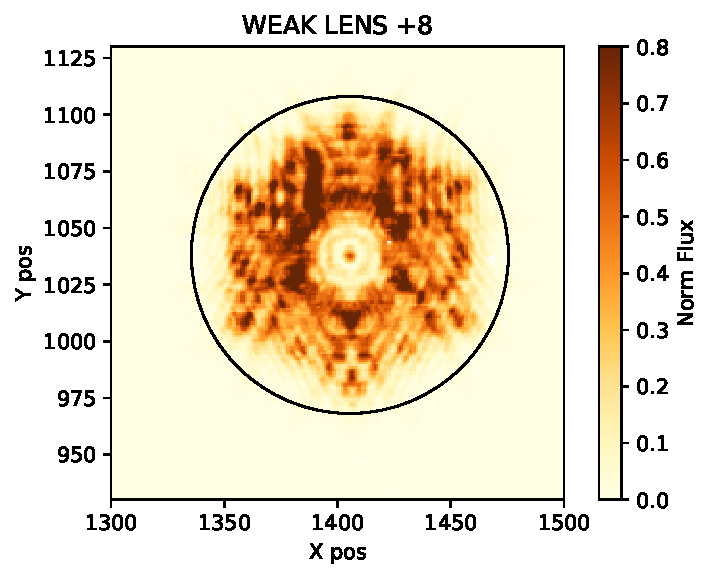
\includegraphics[width=.49\columnwidth]{wlp8_psf.pdf}
\caption{Weak Lans +8 PSF during CV3 testing.
The central peak is used for centroiding, while the entire PSF is used for aperture photometry.
A 70 pixel radius aperture (shown here is a black circle) is used for the source aperture.}\label{fig:WLP8PSF}
\end{figure}

A series of detector stability tests was performed using this +8 wave weak lens and 1.55 $\mu$m LED in a few different modes.
A time series of all possible modes is shown in Figure \ref{fig:CV3longTser}.
The full frame modes (FULL1 through FULLQ) used 2 samples of the ramp for integration times of 21.5 seconds whereas the subarrays were tuned to have a similar integration time (21.3 sec for 20 Groups of a 320$\times$320 subarray and 25.1 seconds for 6 groups of a 640$\times$640 subarray).
This ensured that during these 4 different types of subarray/full frame window sizes, the well depths achieved were similar.

It is apparent from Figure \ref{fig:CV3longTser} that the WLP8SUB test with a 320$\times$320 subarray and 20 groups of the ramp has smaller scatter than the FULL1 through FULLQ tests.
After removing a linear fit to the time series (to account for long term trends in the lamp), the standard deviation of the WLP8SUB data is 500 ppm whereas the FULL tests range from 1020 to 1540 ppm.
For the FULL 2048$\times$2048 pixel integrations with 2 groups up the ramp, the count rate of photons is calculated in each pixel by subtracting the two groups (ie two reads for this RAPID mode) from each other and dividing by the group time (time between these two reads for this RAPID mode).
For the WLP8SUB mode, a linear least squares fit is performed to the groups as a function of time and the slope of this line is the count rate on a pixel.
The large number of groups used to fit this line ensures that the read noise is reduced by $\sim 1/\sqrt{N_G}$, where $N_G$ is the number of groups.

There are two explanations for why the WLP8SUB mode shows less scatter than the FULL modes, 
\begin{enumerate}[noitemsep]
	\item The reduction of read noise improves the stability of the signal and\label{item:readNReasonCV3subFull}
	\item That the lamp is variable on short time scales of a frame (10.74 seconds).\label{item:lampReasonCV3subFull}
\end{enumerate}
The read noise of a pixel is $RN_1 \approx$ 15 e$^-$ for the short wavelength arrays\footnote{https://jwst-docs.stsci.edu/display/JTI/NIRCam+Detector+Performance} in this test.
If this is uncorrelated across the 70 pixel aperture source radius, the read noise from two groups  (correlated double sampling) on the total aperture is $RN_{tot} = \sqrt{N_{s,px}} RN_{CDS} = \sqrt{\pi} r_{s,px} RN_{CDS}$ = 124 * 15 e$^-$ = 1861 e$^- \approx 930 $DN.
This amounts to 25 ppm, which is a small compared to the photon noise (113 ppm).
Furthermore, the read noise for 20 groups is $RN_{20} \approx 6e^-$ would ammount to a 10 ppm, so a difference from the CDS readout of only 15 ppm. {\textbf{\textcolor{red}{(Note, here I have used the effectice read noise for 90 groups on JDox, but should correct to 20 groups)}}
This is dramatically smaller than the observed difference in standard deviation (500 ppm in subarray with 20 groups and 1020-1540 ppm in full frame in 2 groups).
However, if there are correlated components to the read noise in this large aperture, the read noise could be higher.

Under scenario \ref{item:lampReasonCV3subFull}, the short timescale variations of efficiently averaged out by sampling the reads multiple times up the ramp.

\textcolor{red}{To Do: Look at dark frames to measure how correlated the read noise is spatially (certainly the 1/f noise should be correlated}

\begin{figure}[!hbtp]
\centering
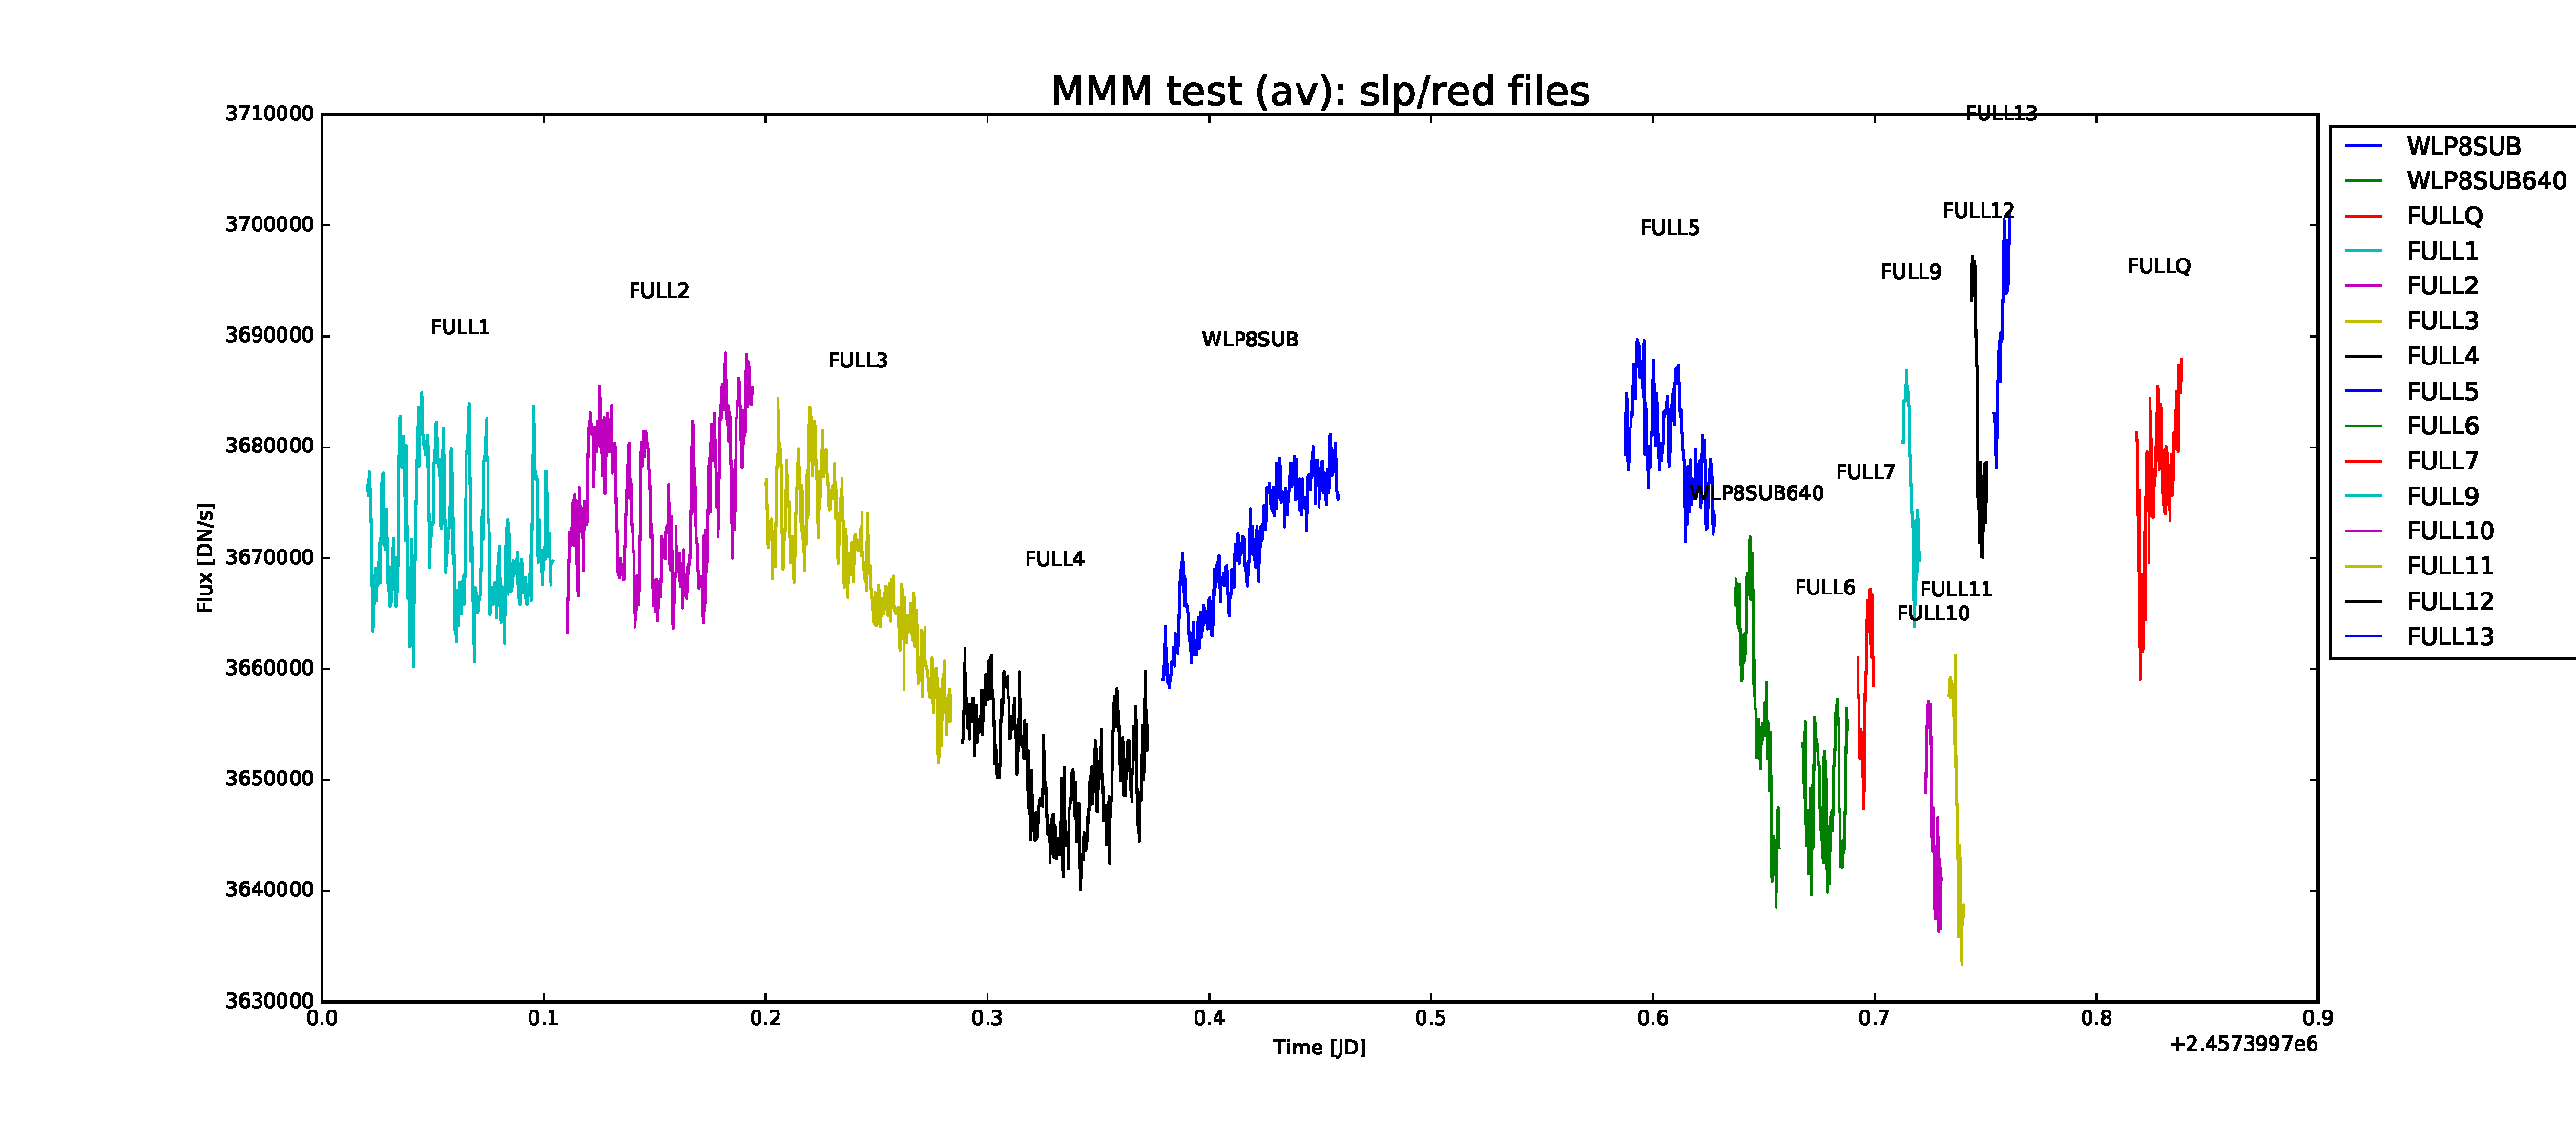
\includegraphics[width=.99\columnwidth]{plot_mmm.pdf}
\caption{Time Series plot through the CV3 photometric stability campaign.
All test shown above were using the Weak Lens +8 mode, with a PSF as shown in Figure \ref{fig:WLP8PSF}.
13 tests (FULL1 through FULLQ) are all in full frame mode, while WLP8SUB used a 320$\times$320 subarray and WLP8SUB640 used a 640$\times$640 subarray.
The WLP8SUB showed the smallest standard deviation of any testof any NIRCam mode explored.}\label{fig:CV3longTser}
\end{figure}

\subsection{Lessons Learned from CV3 Tests}\label{sec:CV3Lessons}
Although the light curves from the CV3 stability tests were not able to achieve photon-limited performance to study the precision of transit and eclipse spectroscopy, there were some lessons learned from this data.
We were able to determine the best practices for the pipeline and analysis by running the raw data through the pipeline and changing the steps to produce light curve.
We experimented with the methodology for turning raw detector reads up the ramp into count rates on the detector, the intrapixel capacitance (IPC) correction, flat fielding, reference pixel correction and detector non-linearity.
After the calibrated images are created, we experimented with different types of aperture photometry including different geometries, background calculations and aperture sizes.

After experimenting with these configurations, we find the following pipeline steps are important:
\begin{itemize}
	\item Fitting a line up the ramp gives superior results to subtracting the last and first pairs of read (as expected by reducing the photon noise)
	\item Centering the aperture with the central spot inside the hexagon is important to conserve the flux within the aperture
	\item Row-by-row subtraction (along the detector's fast-read direction) gives superior background subtraction to traditional aperture photometry (using the mean or robust average value in a background annulus)
	\item Aperture sizes for the source at ~70 pixels, outside the hexagon, gave the best precisions
	\item An annulus aperture on the source (including the inner and outer edges of the hexagonal PSF) usually gives the best precision light curves
\end{itemize}

We also found reduction steps that had very little impact on the final photometric precision including
\begin{itemize}
	\item IPC corrections ($\lesssim 0.01$ ppm)
	\item Flat-fielding ($\lesssim 0.3$ ppm)
\end{itemize}
We summarize the lessons from the tests here.

\subsection{OTIS Tests}

A series of NIRCam stability tests were carried out while the entire JWST telescope system was placed in a tall vacuum chamber at NASA Johnson.
However, there is no feasible way to place a point source lamp at infinity to simulate the imaging of astrophysical objects onto a JWST instrument, so an alternate lamp setup is used.
During these tests, there were two configurations 1) the ``half pass" tests where lamp sources within the optical system and 2) ``pass and a half" tests where the a lamp source within the optical system bounces light off the secondary, primary, flat mirrors mounted on the chamber's ceiling and then through the entire telescope and instrument chain.

The OTIS testing included a time series mode similar to the grism time series template used in orbit for transiting planets.
Figure \ref{fig:otisPSFs} shows the point spread functions for the OTIS tests that simultaneously illuminated the short wavelength and long wavelength channels.
The ``O9'' supercontinuum illuminated the detector over a wide wavelength range from 2.5 to 4.1$\mu$m.
A small fraction of the light is emitted at wavelengths shorter than 2.5 $\mu$m, which is sufficient to illuminate the short wavelength detector to peak counts of $\sim 260$DN per exposure.
Meanwhile, the peak of the grism is $\sim$ 26,000 DN.
This lamp configuration was a pass and a half test, which suffered from the vibrations and oscillations of the suspension system, which can be perturbed by motors such as vacuum pumps.

The point spread function through the weak lens and optical setup create a very unusual point spread function for the short wavelength channel, shown in Figure \ref{fig:otisPSFs} that has multiple clumps of emission.
We perform aperture photometry on a knot of emission at (1090 px, 230 px) for the short wavelength detector.
This knot is concentrated enough to fit with a 2D Gaussian and centroid this Gaussian to ~0.2 pixels, which can be used to track the motions of the PSF due to the oscillations
For the long wavelength detector, we initially extract a box aperture to create a broadband light curve.


\begin{figure*}
\gridline{\fig{wlp8_otis_psf.pdf}{0.7\textwidth}{WLP8 Image} }
\gridline{\fig{{grism_otis_psf.pdf}}{0.7\textwidth}{Grism Image}}
\caption{Median images of the short wavelength (SW) weak lens mode and long wavelength (LW) grism spectroscopy that were used simultaneously in a grism time series stability test.
Due to the OTIS optics setup, the short wavelength WLP8 image does not nearly represent the hexagonal PSF from CV3 (Figure \ref{fig:WLP8PSF}) or flight.
}\label{fig:otisPSFs}
\end{figure*}

\begin{figure*}
%\gridline{\fig{tser_LW_OTIS.pdf}{0.99\textwidth}{WLP8 Image} }
\gridline{\fig{tser_LW_OTIS.pdf}{0.6\textwidth}{Grism Time Series}}
\caption{Time series of the simultaneous SW/LW Time Series Stability test
}\label{fig:otisLWSWtser}
\end{figure*}


As with the CV3 tests in Section \ref{sec:CV3Lessons} and Figure \ref{fig:CV3longTser}, we found the highest precision lightcurves when using subarray read configurations.
Figure \ref{fig:OTISsubarrays} shows the many subarrays explored in a set of time series.
As the number of reads up the ramp becomes larger and larger, the standard deviation increases.
This would be expected if the read noise contributed significantly to the standard deviation so that ramp fitting decreases the read noise.
The perplexing thing is, though, that this is even true if we throw away all the intermediate reads.
That is, with all readout modes, count rate (ie. slope image is approximated by the last subtracted by the first read.
Here the number of reads in between these is irrelevant.
A possible way to explain the superior standard deviation for the smallest 2048$\times$64 subarray is not that more reads increase precision but rather the small subarray has a smaller contribution from spatially correlated noise.
When larger frames are read out, for example, the 1/f noise becomes increasingly uncorrelated from read to read.\textcolor{red}{Wrote this when very tired. Is this correct and logical?}

Note that the integration times are different for these 4 tests. They are 39.9, 39.9, 32.3, 31.8 and 32.2 for the 64-STRIPE, 128-STRIPE, 256-STRIPE, 256-WIND and FULLFRAME respectively. Perhaps the lamp has oscillations on a timescale that are averaged out efficiently at 39.9 seconds but not 32.3 seconds?

\begin{figure}[!hbtp]
\centering
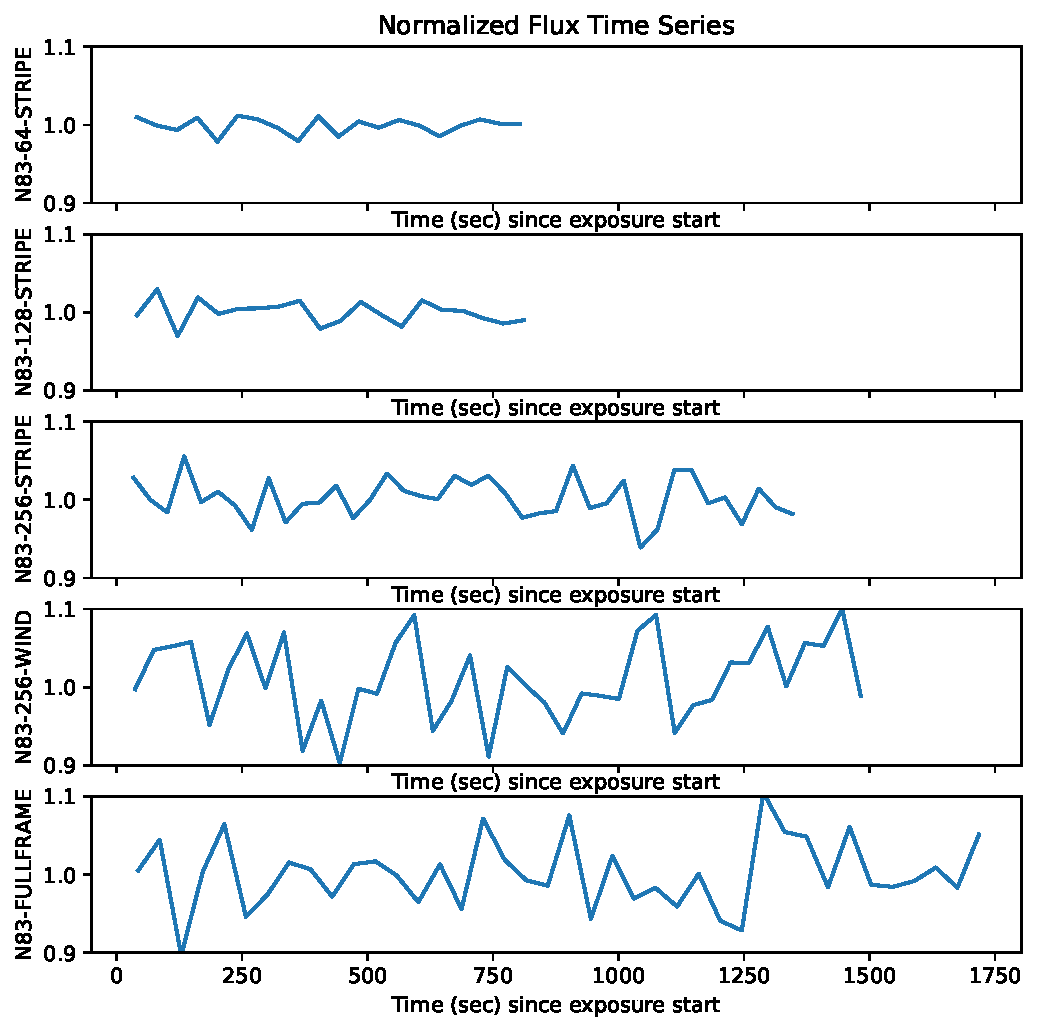
\includegraphics[width=.5\columnwidth]{subarray_config_tser.pdf}
\caption{A variety of subarrays in the OTIS stability tests were read out with similar integration times (32 to 39 seconds) to compare relative precision of the read modes. 
The time series are ordered vertically in increasing frame duration (and decreasing number of groups up the ramp) toward the bottom.
The standard deviation decreases as the number of groups up the ramp becomes more numerous.}\label{fig:OTISsubarrays}
\end{figure}

\subsection{GL Dewar Tests}

The GL dewar, located at the University of Arizona, is a laboratory setup for assessing NIRCam flight and spare detectors.
The key difference with the Asic dewar discussed below is that the detector readout electronics are completely different, using a Leach system that is operated outside of the dewar as opposed to the Asic, which is lives right next to the detectors.
The GL dewar detector stability tests are helpful in isolating noise sources that arise from the detectors versus the readout electronics.

An LED illumination source is pointed at the detectors and the arrays are read out in subarray mode.
Figure \ref{fig:GLtSeries} shows the detector subarray illumination as well as two apertures that were used for time series photometry.
The first handful of frames show an initial "warmup" period lasting about 9 seconds.
This quickly stabilizes to a 1200 ppm level likely dominated by lamp variations.
If one divides the two apertures by each other, the resulting time series is very flat and stable to with 260 ppm.
When binning the data into 2.5 minute increments, the standard deviation is only 51 ppm.


\begin{figure*}
\gridline{\fig{ap_labels_S02illum_GLrun104.pdf}{0.32\textwidth}{Apertures}
		\fig{raw_tser_phot_S02illum1miAll_GLrun104.pdf}{0.32\textwidth}{Raw time series}
		\fig{refcor_phot_S02illum1miAll_GLrun104.pdf}{0.32\textwidth}{Ratio Time Series}}
\caption{The precision of this short-duration GL dewar test was the extremely high at $\sigma=$240 ppm after stabilization.
}\label{fig:GLtSeries}
\end{figure*}

\subsection{Asic Dewar Tests}

%% If you wish to include an acknowledgments section in your paper,
%% separate it off from the body of the text using the \acknowledgments
%% command.
\acknowledgments

\section{Expected In-Flight Performance with JWST}

\section*{acknowledgements}
MCMC fitting makes use of \texttt{emcee} \citep{foreman-mackey2013emcee} and the covariance plot was made with \texttt{corner.py} \citep{foremanCorner}.
Funding for the E Schlawin is provided by NASA Goddard Spaceflight Center.
This research has made
use of the Exoplanet Orbit Database and the Exoplanet Data Explorer at \url{http://exoplanets.org}; SIMBAD database, operated at CDS, Strasbourg,
France; NASA's Astrophysics Data System Bibliographic
Services; the M, L, T, and Y dwarf compendium
housed at \url{http://DwarfArchives.org}; the SpeX Prism
Libraries at \url{http://www.browndwarfs.org/spexprism}; and the \texttt{astropy} package \citep{astropy2013}. 
The authors wish to recognize and acknowledge the very significant cultural role and reverence that the summit of Mauna Kea has always had within the indigenous Hawaiian community. We are most fortunate to have the opportunity to conduct observations from this mountain.

%% To help institutions obtain information on the effectiveness of their 
%% telescopes the AAS Journals has created a group of keywords for telescope 
%% facilities.
%
%% Following the acknowledgments section, use the following syntax and the
%% \facility{} or \facilities{} macros to list the keywords of facilities used 
%% in the research for the paper.  Each keyword is check against the master 
%% list during copy editing.  Individual instruments can be provided in 
%% parentheses, after the keyword, but they are not verified.

\vspace{5mm}
\facilities{HST(WFC3), IRTF(SpeX)}

%% Similar to \facility{}, there is the optional \software command to allow 
%% authors a place to specify which programs were used during the creation of 
%% the manusscript. Authors should list each code and include either a
%% citation or url to the code inside ()s when available.

\software{astropy \citep{astropy2013}, 
          \texttt{emcee} \citep{foreman-mackey2013emcee}, 
          \texttt{batman} \citep{kreidberg2015batman},
          \texttt{spiderman} \citep{louden2017spiderman},
          \texttt{pynrc} \url{https://github.com/JarronL/pynrc},
          \texttt{emcee} \citep{foreman-mackey2013emcee}
           }

%% Appendix material should be preceded with a single \appendix command.
%% There should be a \section command for each appendix. Mark appendix
%% subsections with the same markup you use in the main body of the paper.

%% Each Appendix (indicated with \section) will be lettered A, B, C, etc.
%% The equation counter will reset when it encounters the \appendix
%% command and will number appendix equations (A1), (A2), etc. The
%% Figure and Table counter will not reset.

\appendix

%\section{Extra Info}

%% The reference list follows the main body and any appendices.
%% Use LaTeX's thebibliography environment to mark up your reference list.
%% Note \begin{thebibliography} is followed by an empty set of
%% curly braces.  If you forget this, LaTeX will generate the error
%% "Perhaps a missing \item?".
%%
%% thebibliography produces citations in the text using \bibitem-\cite
%% cross-referencing. Each reference is preceded by a
%% \bibitem command that defines in curly braces the KEY that corresponds
%% to the KEY in the \cite commands (see the first section above).
%% Make sure that you provide a unique KEY for every \bibitem or else the
%% paper will not LaTeX. The square brackets should contain
%% the citation text that LaTeX will insert in
%% place of the \cite commands.

%% We have used macros to produce journal name abbreviations.
%% \aastex provides a number of these for the more frequently-cited journals.
%% See the Author Guide for a list of them.

%% Note that the style of the \bibitem labels (in []) is slightly
%% different from previous examples.  The natbib system solves a host
%% of citation expression problems, but it is necessary to clearly
%% delimit the year from the author name used in the citation.
%% See the natbib documentation for more details and options.

\bibliographystyle{apj}
\bibliography{this_biblio}

%% This command is needed to show the entire author+affilation list when
%% the collaboration and author truncation commands are used.  It has to
%% go at the end of the manuscript.
%\allauthors

%% Include this line if you are using the \added, \replaced, \deleted
%% commands to see a summary list of all changes at the end of the article.
%\listofchanges

\end{document}

% End of file `sample61.tex'.
